\chapter{Preprocessing and Transformation}
\label{cha:preprocessing_transformation}

In total, two datasets were used to create features for testing the different classifiers:
\textit{movies\_metadata.csv} and \textit{credits.csv}. The dataset \textit{movies\_metadata.csv} contains 45,463 rows and 23 columns excluding the id-column. The dataset \textit{credits.csv} contains 45,463 rows and 2 columns excluding the id-column. Based on the assumptions that budget and revenue were crucial numbers, the release year has an impact on those numbers and the genre, the production country such as production company, the spoken languages, the runtime and the fact whether a movie belongs to a collection or not are further important information, all others columns were dropped out from the \textit{movies\_metadata.csv}. \textbf{Nicht gerade wisschenschaftlich hier} Figure \ref{img:mm_columns} gives an overview which information was kept.

The reason why information, which could have been potentially interesting, had to be dropped, was mainly for time reasons. Preprocessing took about 70\% of the timeperiod\footnote{Mainly due to the fact that heaps of problems arose from the dataset, which can be read in chapter \ref{cha:data_selection}.} of the whole project. Thus, the team was able to focus on preprocessing of mentioned columns. Still, chapter \ref{cha:interpretation_evaluation} provides a prospect, which steps were possible, if a larger timeframe was dedicated to this project.

After dropping out information, eleven columns remained. Combined with the two columns from the \textit{credits.csv} dataset, thirteen columns were used as a basis to create features for finding the best performing classifiers.

\begin{figure}
	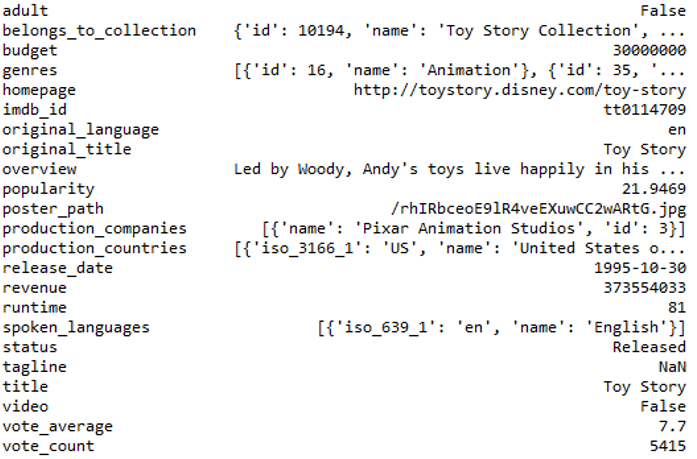
\includegraphics[width=\textwidth]{images/3_metadata_columns.png}
	\caption{Dropped columns of \textit{movies\_metadata.csv}. All kept columns are marked in yellow}
	\label{img:mm_columns}
\end{figure}

In order to transform the data into a suitable representation for forecasting a movie's success, preprocessing was mandatory. All preprocessing steps included either the following:
\begin{itemize}
	\item Merging of columns
	\item Binning of features
	\item Extracting information out of columns
	\item One hot encoding
	\item Normalizing
\end{itemize}



\begin{figure}
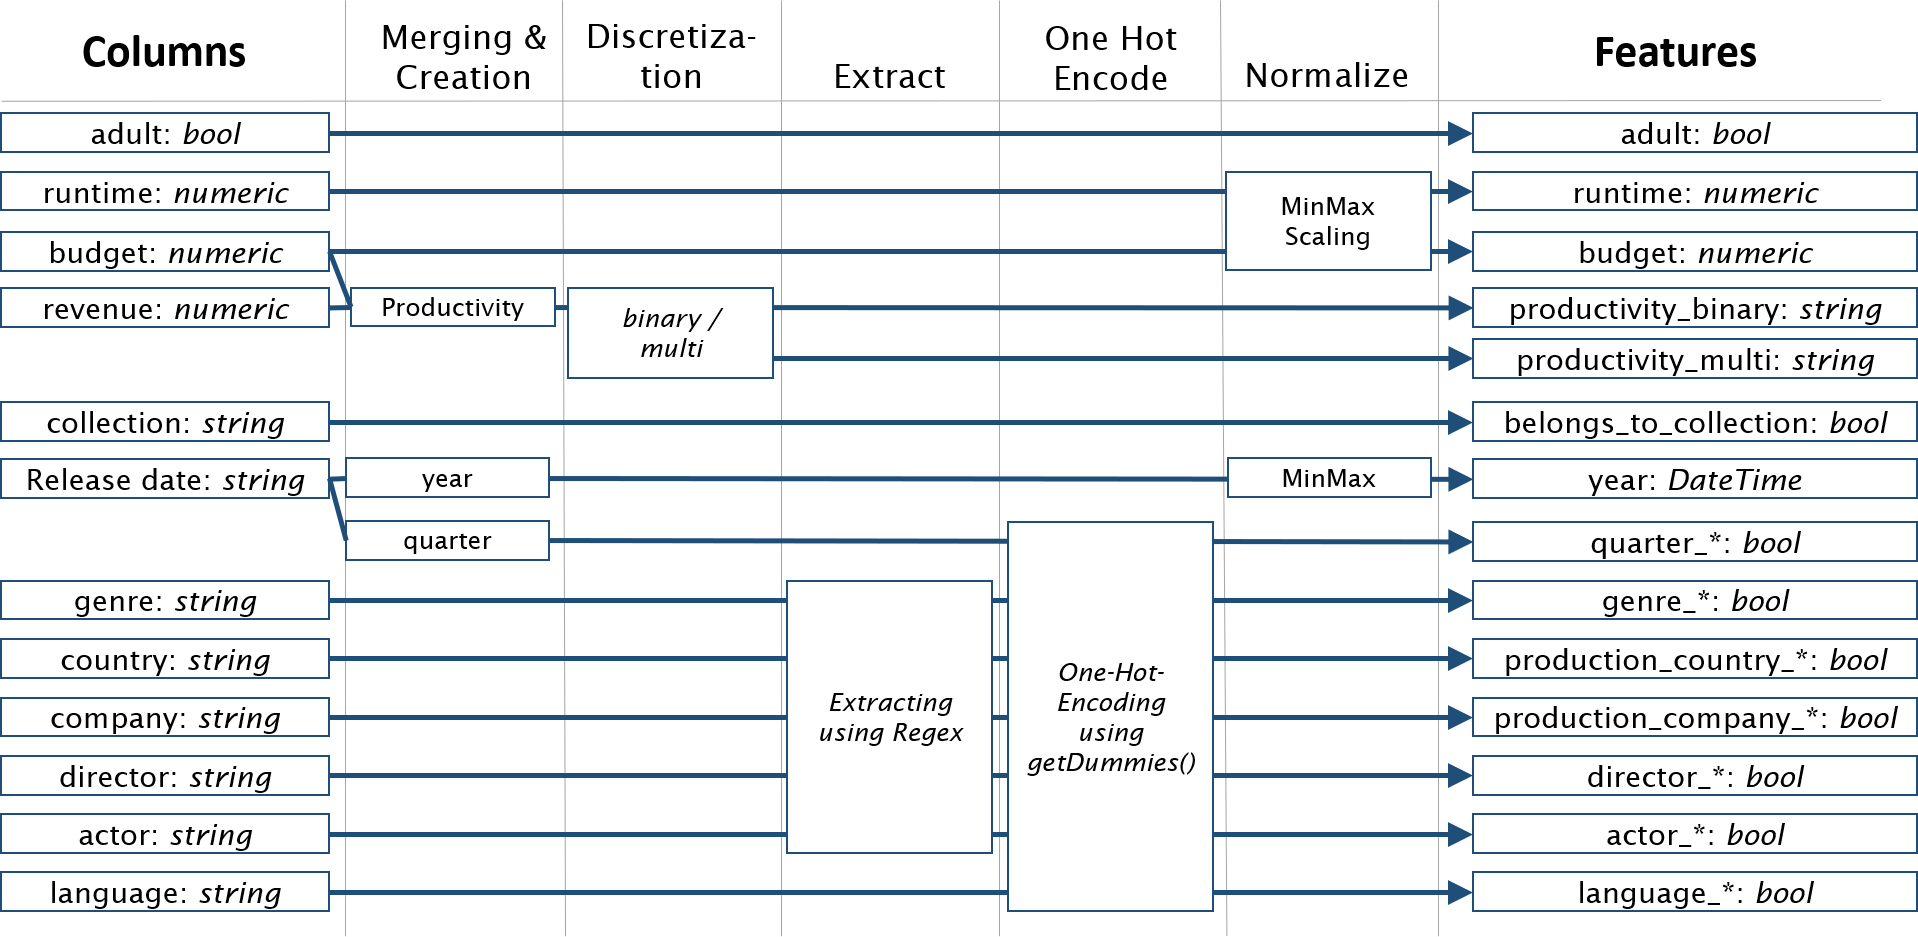
\includegraphics[width=\textwidth]{images/3_features.png}
\caption{Features created during preprocessing}
\label{img:features}
\end{figure}


\begin{itemize}
	\item Transform data into a representation that is suitable for the chosen data mining methods
	\begin{itemize}
		\item number of dimensions
		\item scales of attributes (nominal, ordinal, numeric)
		\item amount of data (determines hardware requirements)
	\end{itemize}
	\item Methods
	\begin{itemize}
		\item Aggregation, sampling
		\item Dimensionality reduction / feature subset selection
		\item Attribute transformation / text to term vector
		\item Discretization and binarization
	\end{itemize}
	\item Good data preparation is key to producing valid and reliable models
	\item Data preparation estimated to take 70-80\% of the time and effort of a data mining project!
\end{itemize}


\section{Preprocessing steps according to Python script}

\section{A list of problems we encountered}
\begin{enumerate}
	\item \textbf{list further problems we had and solved!}
	\item Prod. Comp.: Same prod. company named differently -> using Regex to solve (Steffen)
	\item dataset: 5 datasets have duplicates
\end{enumerate}
